% GUIDA VELOCE:
% --------------------------------------------------------------------
% X INIZIA UN UNOVO CAPITOLO:
% \chapter{??? NOME CAPITOLO}}
% \section{ ?? }
% \subsection{ ?? }
%
% --------------------------------------------------------------------
% PAROLA CONTENUTA NEL GLOSSARIO:
% scrivere la parola seguita da $^g$
% esempio: User$^g$
%
% --------------------------------------------------------------------
% PER ANDARE A CAPO SENZA RIENTRO INSERIRE:
% \\
%
% --------------------------------------------------------------------

% GRASSETO:
% \textbf{parola}
%
% --------------------------------------------------------------------
% CORSIVO:
% \emph{parola}
% --------------------------------------------------------------------
% PER SCRIVERE IN ROSSO:
% \red{parola}
%
% --------------------------------------------------------------------
% PER SCRIVERE TRA VIRGOLETTE
% ''parola''
%
% --------------------------------------------------------------------
% PER EVITARE IL RIENTRO AUTOMATICO DI UN CAPOVERSO:
% \noindent testo....
%
% --------------------------------------------------------------------

% PER SCRIVERE CARATTERI PARTICOLARI COME: { } _ ecc.. SCRIVERLI PRECEDUTI DA \
% ES: \{ \_
%
% --------------------------------------------------------------------
% X INSERIRE UN LINK:
% \url{http://www.math.unipd.it/~tullio/IS-1/2011/Progetto/C3.pdf}
%
% --------------------------------------------------------------------
% PER COMMENTARE INTERE PARTI:
% \comment{ comment }
%
% --------------------------------------------------------------------
% PER SCRIVERE NOTE DURANTE IL TESTO:
% parola \footnote{ note riguardanti la parola }
%
% --------------------------------------------------------------------
% PER SCRIVERE CODICE SORGENTE:
%
% \lstset{language=c++,
% stringstyle=\color{blue}\textrm,
% commentstyle=\rmfamily, numbers= none}

% \begin{lstlisting}
% CODICE
% \end{lstlisting}
%
% --------------------------------------------------------------------
% !!!!!!!! PER COSE + COMPLESSE VEDI: !!!!!!!!!!!!!!!!!!!!!!!
% !!!!!!!! PMAC/latex/GUIDA LATEX!!!.tex !!!!!!!!!!!!!!!!!!!!!!!

% per tutto il resto chiedi a lory prima di fare/scrivere cazzate !!!!!!!!!!



\documentclass[10pt,a4paper]{article}

\usepackage[italian]{babel}
\usepackage[T1]{fontenc}
\usepackage[utf8x]{inputenc} % uso utf8x xk x linux, mentre latin1 è per windows
\usepackage{lmodern} %insieme di font molto completo consigliato da LatexFacile pg13 in basso
\usepackage{microtype} %migliora riempimento delle righe. vedi LatexImpaziente pg41
%attiva il rientro di ogni prima riga di ogni sezione: capitolo,paragrafo ecc. vd LatexImpaziente pg41
\usepackage{indentfirst}
\usepackage{graphicx} % per inseire immagini
\usepackage[usenames,dvipsnames]{color}
\usepackage{lastpage} %serve per poter scrivere page 1 of N
% setta i bordi della pagina: dx e sx 3.2cm di rientro + nel lato di rilagatura rientra di altri 0mm
\usepackage[a4paper,top=2.7cm,bottom=2.7cm,left=2.7cm,right=2.7cm, bindingoffset=0mm]{geometry}
\usepackage{listings} % per inserire codice sorgente
\usepackage{float} % per gestire oggetti flottanti ( es immagini tabelle posizionebili con "H" che forza il posizionamento nel punto specifico )

% serve per creare tabelle lunghe + di una pagina con \begin{longtable} (vd Tabelle.pdf pg11-12)
\usepackage{longtable}

\usepackage{fancyhdr} % per impostare lo stile della pagina più personalizzato, + fancyhdr ( per regolare testatina e piè di pagina ) vedi itfancyhrd


\pagestyle{fancy}
% settaggi di pagestyle(fancy)
\lhead{
\includegraphics[scale=0.20]{images/nastro}}
%\chead{}
\rhead{\textbf{Tecnologie Web \\ Data: \DataRilascio}}
\lfoot{\NomeDocumento}
\cfoot{}
\rfoot{ \textbf \thepage\ of \pageref{LastPage}}
\renewcommand{\footrulewidth}{0.4pt}

%ridefinisco il plain per cosare l'indice (a questo punto si potrebbe lasciare tutto il documento in plain
\fancypagestyle{plain}{
%\lhead{\includegraphics[scale=0.20]{SevenFold_small}}
%\chead{}
\rhead{\textbf{{ Tecnologie Web}}}
\lfoot{\NomeDocumento}
\cfoot{}
\rfoot{ \textbf \thepage\ of \pageref{LastPage}}
\renewcommand{\footrulewidth}{0.4pt}
}

% da ultimo:
\usepackage{hyperref} %x l'interpretazione di indirizzi o link ipertestuali (vd LatexImpaziente pg47 )
\hypersetup{backref, colorlinks=true, linkcolor=black, urlcolor=black}

\usepackage{url} % x l'interpretazioni di internet o link ipertestuali (vd LatexImpaziente pg47 )
%\UrlFont{color =blue}
%\urlstyle{helvetic}

% Define a new 'leo' style for the package that will use a smaller font.
\makeatletter
\def\url@leostyle{%
  \@ifundefined{selectfont}{\def\UrlFont{\sf}}{\def\UrlFont{\small\ttfamily}}}
\makeatother
%% Now actually use the newly defined style.
\urlstyle{leo}


\newcommand{\mail}[1]{\textcolor{Black}{ \texttt{#1}}} %per interpretare mail (vd LatexImpaziente pg47 )
\newcommand{\cambiaFont}[2]{{\fontencoding{T1}\fontfamily{#1}\selectfont#2}}
\newcommand{\red}[1]{ \textcolor{red}{#1} } % per scrivere testo in rosso
\newcommand{\blue}[1]{ \textcolor{blue}{#1} } % per scrivere testo in blu
\newcommand{\comment}[1]{} % per inserire commenti

\newcommand{\attribute}[2]{ \item[\textcolor{PineGreen}{ \texttt{#1}}] \textcolor{PineGreen}{\texttt{#2\\}}\ \ \ }
\newcommand{\method}[2]{ \item[\textcolor{MidnightBlue}{ \texttt{#1}}] \textcolor{MidnightBlue}{ \texttt{#2\\}}\ \ \ }

\newcommand{ \class}[1]{ \item[ \textcolor{MidnightBlue}{\texttt{-}}] \textcolor{MidnightBlue}{\texttt{#1}}}
\newcommand{ \classe}[1]{ \noindent \textcolor{MidnightBlue}{\texttt{-}} \textcolor{MidnightBlue}{\texttt{#1}}}

\newcommand{\tab}{\hspace*{1.5em}}


% INSERIRE QUI IL NOME DEL DOCUMENTO SEGUITO DA UNO SPAZIO
% ( così il nome si imposta in automatico nelle varie ricorrenze standard)
\newcommand{\NomeDocumento}{Relazione progetto: \textit{"AllStreaming"}}

% INSERIRE QUI LA DATA DEL RILASCIO DELLA VERSIONE ATTUALE
\newcommand{\DataRilascio}{19-06-2012}

\newcommand{\serie}{\textit{Serie Tv}}
\newcommand{\film}{\textit{Film}}
\newcommand{\all}{\textit{AllStreaming}}
\newcommand{\n}{\noindent}


\begin{document}


% --------------------------------------------------------------------

% TITOLO ( 1° pagina)

\vspace*{1cm}
\begin{center}

%\cambiaFont{Cyklop}{Sevenfold}
%\cambiaFont{fve}{\Huge{Sevenfold}}


\vspace{1.5cm}

\textit{\Huge{Relazione per il progetto \\del corso di Tecnologie Web:}}\\
\vspace{1.3cm}
\cambiaFont{fve}{\Huge{\color{blue}{""AllStreaming""}}}
\vspace*{1.8cm}

\large{Università degli studi di Padova\\
anno accademico 2011-2012}

\vspace*{1cm}


\includegraphics[scale=0.35]{images/nastro10e.png}

\end{center}


% --------------------------------------------------------------------

% INFORMAZIONI DEL DOCUMENTO ( 1° pagina)

\vspace*{2cm}
\begin{center}

\begin{tabular}{ r | l }
\multicolumn{2}{c}{\textbf{\Large{Informazioni del documento}} }\\
\hline
\rule[-1.5mm]{0mm}{0.7cm}
\textbf{Titolo del documento} & \NomeDocumento\\
\rule[-1.5mm]{0mm}{0.5cm}
\textbf{Date}& \DataRilascio\\
\rule[-1.5mm]{0mm}{0.5cm}
\textbf{Autori}& \underline{Lorigiola Giacomo} [ 592992 ]\\
& \underline{Spiga Gabriele} [592141]\\
& \underline{Luca Guerra} [591394]\\
\rule[-1.5mm]{0mm}{0.5cm}
\textbf{Destinatario}&Prof.essa Ombretta Gaggi\\
\end{tabular}

\end{center}

% --------------------------------------------------------------------

% SOMMARIO ( 2° pagina)

\newpage

\vspace*{0.5cm} % il vertical space va preceduto da una riga vuota!!!
\begin{center}

\textbf{{\Large{Sommario}}}

Questo documento intende presentare una analisi del progetto per il corso di Tecnologie Web intitolato "AllStreaming", giustificando le scelte architetturali e tecnologiche intraprese in corso di progetto.


\vspace*{0.2cm} % il vertical space va preceduto da una riga vuota!!!

\end{center}



% --------------------------------------------------------------------
% INDICI:

\newpage

% INDICE CAPITOLI
\tableofcontents % genera l'indice di tutto il documento

\let\cleardoublepage\clearpage % toglie la pagina bianca dopo l'indice

% INDICE TABELLE
% \listoftables

% INDICE FIGURE
\listoffigures


% --------------------------------------------------------------------

% INTRODUZIONE ( 1° CAPITOLO ) QUESTO CAPITOLO VA MESSO IN OGNI DOCUMENTO!!!!!!!!

\newpage


\section{Introduzione}
Il tema scelto ci sembra quanto mai attuale, in quanto da 3 anni a questa parte sono nati innumerevoli portali che forniscono un servizio simile a quello che proponiamo, costituendo una valida e soprattutto più economica alternativa a tradizionali abbonamenti pay-per-view.
L'obiettivo del sito è fornire un portale unitario per la visualizzazione di link attraverso i quali poter accedere alla visualizzazione in streaming di contenuti video come film o serie Tv.
Gli utenti potranno selezionare il video di loro interesse scegliendo tra quelli disponibili nelle apposite sezioni \film \ e \serie, e seguendo i link riportati, accedere ai più gettonati siti di hosting per la visualizzazione del video scelto.\\
Importante notare che il tutto è perfettamente legale, visto che come specificato nella sezione "Chi Siamo", il sito si limita a reindirizzare l'utente verso i contenuti, i quali non sono ospitati dal server stesso.

\noindent Il sito realizzato è stato caricato nel server di tecnologie-web della facoltà, alle login \textbf{glorigio} e \textbf{lguerra}.\\

\noindent E' possibile accedere al sito oltre che come visitatore, anche come amministratore o utente registrato con le seguenti credenziali:
\begin{itemize}


\item credenziali amministratore del sito:\\
\textit{username:} \textbf{admin}\\
\textit{password:} \textbf{password}
\item credenziali utente registrato:\\
\textit{username:} \textbf{jack}\\
\textit{password:} \textbf{password}\\
\end{itemize}


\section{Considerazioni generali}

Il sito web è stato pensato e realizzato al fine di rendere semplice ed intuitiva la navigazione al suo interno, permettendo così un agevole accesso alle informazini in esso contenute.\\
Questi aspetti fondamentali, che ogni sito ben struttutato dovrebbe avere, possono essere riassunti nei seguenti punti:
\begin{itemize}
\item \textit{reperibilità dei contenuti}
\item \textit{accessibilità}
\end{itemize}

\n La reperibilità dei contenuti è un aspetto fondamentale in quanto permette agli utenti di poter trovare nel minor tempo possibile e nel minor numero di ''click'' possibili le informazioni ricercate rendendo così il sito molto immediato. L'utilizzo ottimizzato delle locandine rende questa operazione molto più semplice\\

\n E' stata posta inoltre particolare attenzione all' accessibilità del sito, dettata dalla considerazione che gli utenti visualizzatori potrebbero essere di svariate tipologie e condizioni fisiche.\\
Gli utenti infatti potrebbero avere disabilità e quindi per esempio difficoltà nell'utilizzo dei normali strumenti come mouse o tastiera, oppure difficoltà visive che richiedono l'utilizzo degli screen reader per effettuare la navigazione internet; sono infatti disponibili funzioni per saltare la lettura dei menu o delle parti di testo che appaiono in ogni pagina, al fine di velocizzare l'accesso ai contenuti veri e propri.\\
Ancora, gli utenti potrebbero accedere al sito attraveso vecchi browser, oppure dispositivi mobili come tablet o smartphone che dispongono di schermi relativamente piccoli per poter visualizzare comodamente il layout completo del sito, per questo sono disponibili diversi fogli di stile. Infatti in fase di progettazione sono state tenute completamente separate le parti di struttura e contenuto da quelle di presentazione. \\


\section{Utenti}
Gli utenti che possono visualizzare il sito sono stati suddivisi in tre differenti categorie:
\begin{itemize}
\item \textbf{utente visitatore}
\item \textbf{utente registrato}
\item \textbf{admin}
\end{itemize}

\n Al sito può accedere liberamente qualsiasi utente che desidera farne uso, non è infatti richiesta alcuna iscrizione al sito per potervi accedere. E' previstà però una limitazione per gli utenti visitatori che non sono registrati e autenticati nel sito, i quali non possono nè visualizzare i commenti ai video rilasciati dagli utenti registrati, nè vedere i profili di tali utenti.\\
L'utente registrato è l'utente che ha deciso di iscriversi al sito attraverso l'apposita sezione di registrazione, creando il proprio profilo personale.\\
E' previsto inoltre un utente admin che ha il compito di manutentore del sito; tra le varie funzionalità egli può eliminare utenti iscritti, inserire film serie Tv, aggiungere a questi informazioni correlate come stagioni, episodi e link per la visualizzazione in streaming ed eliminare eventuali commenti inopportuni.


\section{Pagine del sito}
Per garantire una navigazione semplice e veloce, le pagine sono state suddivise per argomenti e in modo gerarchico garantendo così un accesso immediato alle sezioni desiderate.\\
Inoltre in base alla tipologia di utente che accede al sito, potranno essere visualizzate differenti pagine.\\

\subsection{Suddivisione delle pagine}
Di seguito viene presentata in modo schematico la suddivisione della pagine alle quali possono accedervi gli utenti in base alla loro tipologia.

\begin{itemize}

\item \textbf{Suddivisione pagine per utente visitatore:}

\begin{center}
\begin{figure}[H]
\centering
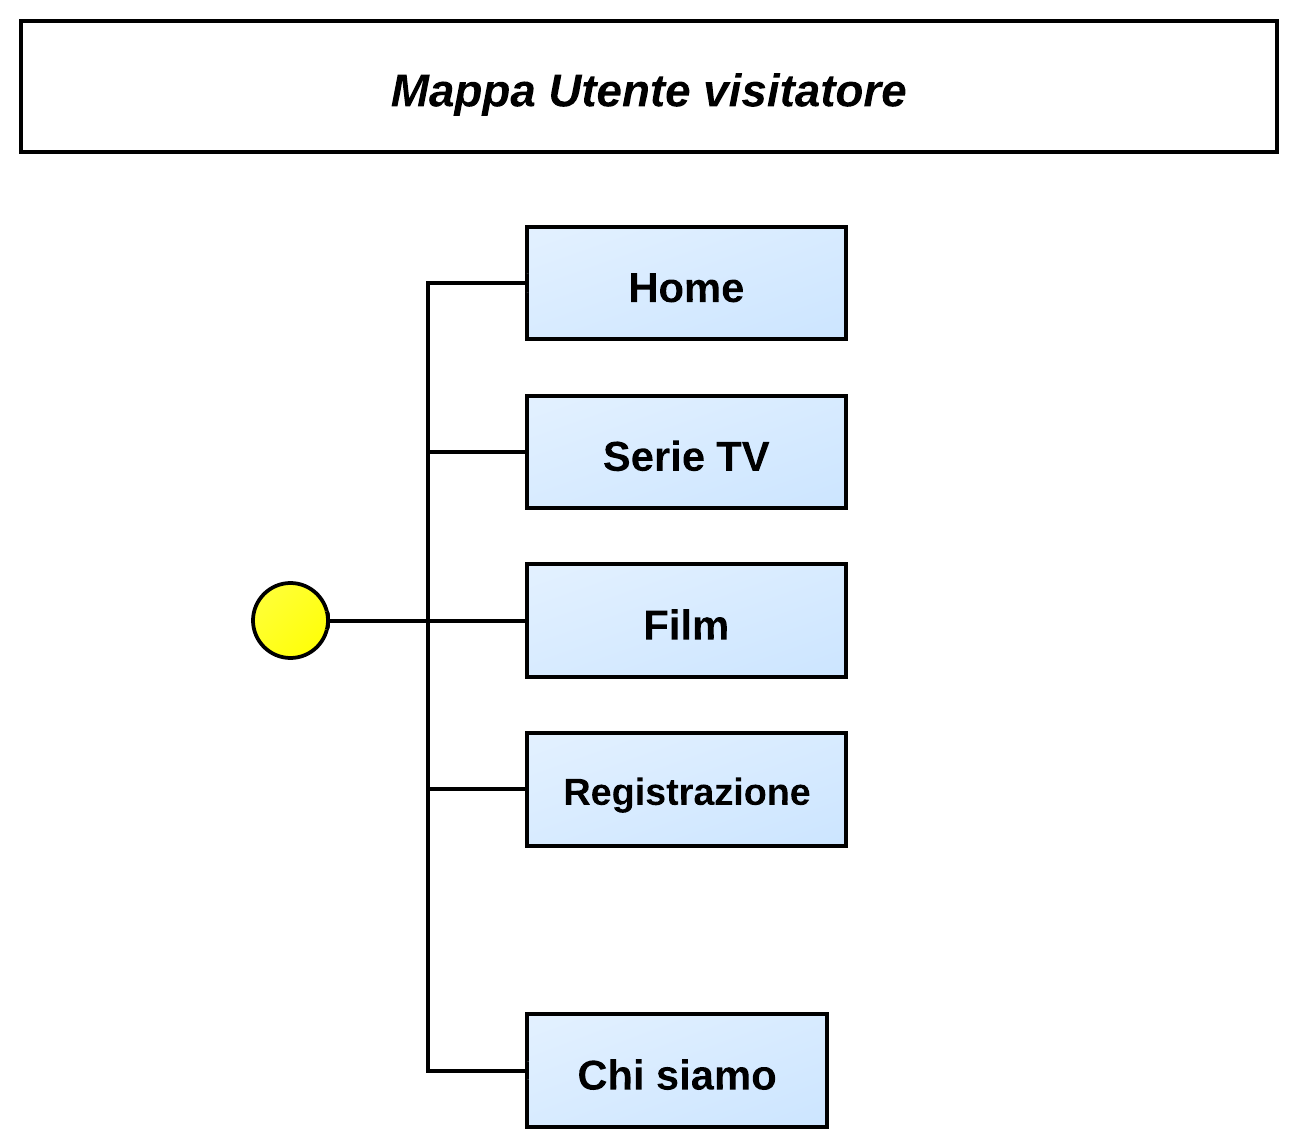
\includegraphics[scale=0.60]{images/mapVisitatore.png}
\caption{Mappa utente visitatore}
\end{figure}
\end{center}


\item \textbf{Suddivisione pagine del sito per utente registrato e admin:}

\begin{center}
\begin{figure}[H]
\centering
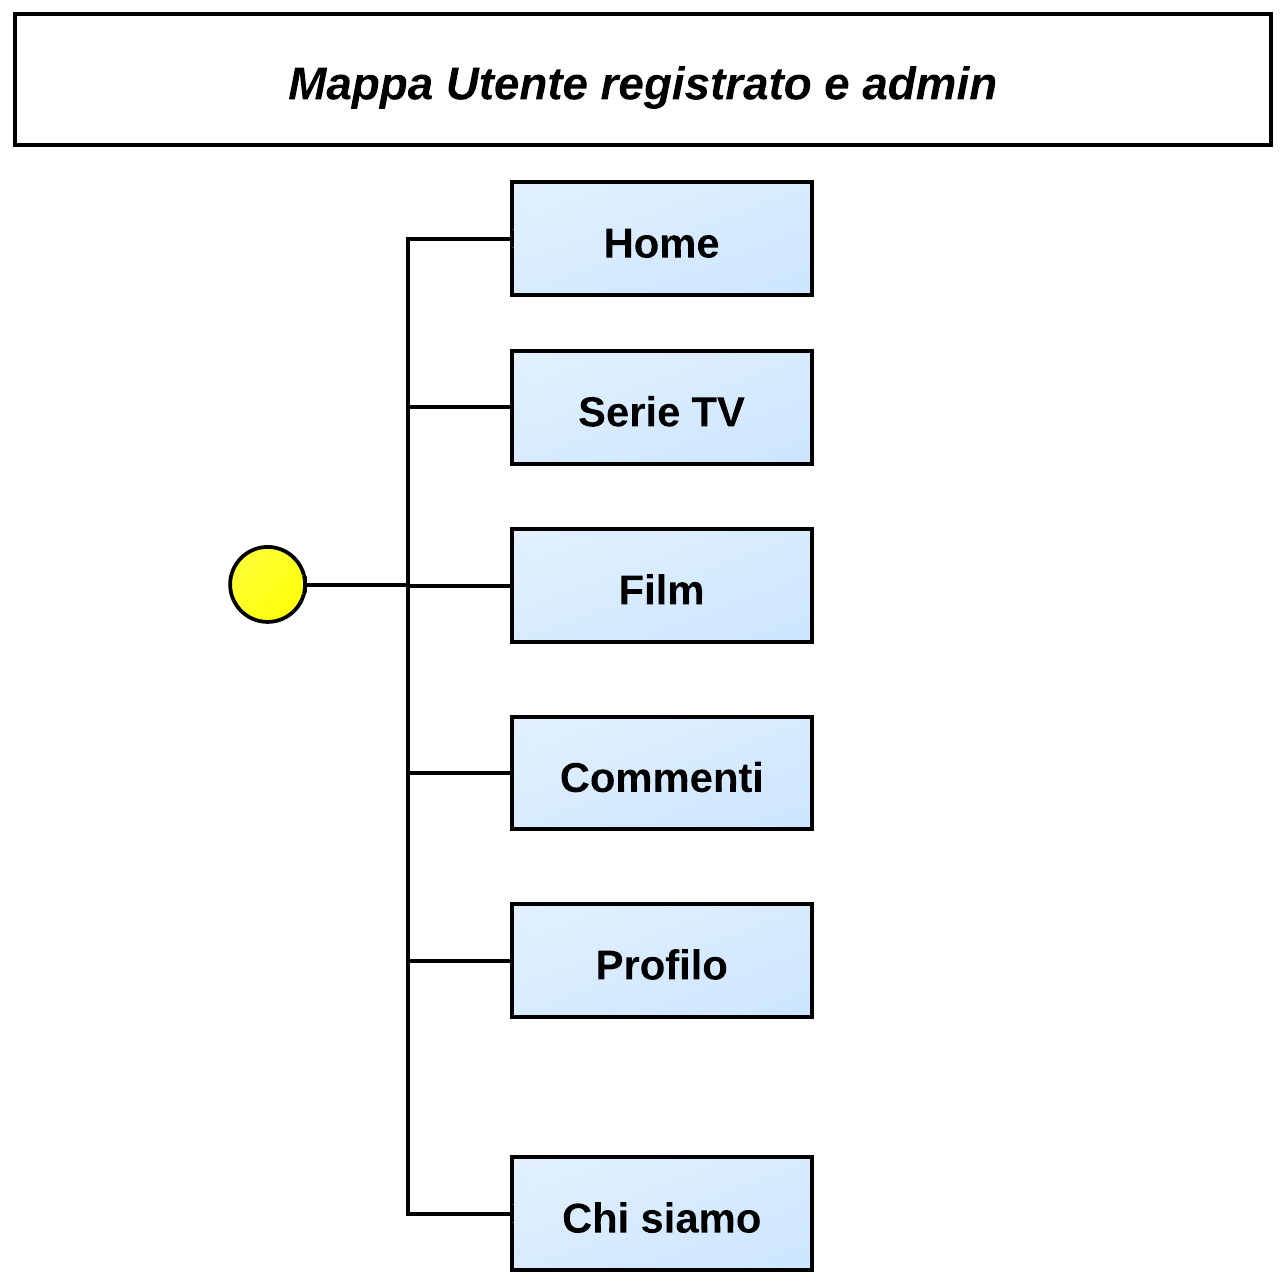
\includegraphics[scale=0.60]{images/mapRegistrato.png}
\caption{Mappa utente registrato e admin}
\end{figure}
\end{center}


\end{itemize}


\subsection{Pagine principali:}
Per ogni pagina del sito, viene di seguito posta una presentazione e descrizione; in base alla tipologia di utente, una determinata pagina può non essere visibile, o visibile in modo differente.

\begin{itemize}
\item \textbf{Home}:\\
Per gli utenti visitatori e registrati questa pagina presenta una anteprima di alcuni film proposti.\\
Per l'utente admin invece questa pagina permette di visualizzare le informazini generali del sito come il numero degli utenti iscritti, il numero di film e serie inserite. Da qui inoltre l'admin ha la possibilità di visualizzare i link alle pagine per l'inserimento di un nuovo film o di una nuova serie.
\item \textbf{Serie Tv}:\\
Questa pagina è medesima per qualsiasi utente, e permette la visualizzazione dell'elenco di tutte le Serie Tv presenti nel sito. Una volta scelta la Serie Tv, cliccandovi si accede alla pagine specifica della serie.
\item \textbf{Film}:\\
Anche questa pagine è edesima per qualsiasi utente, e permette la ricerca un un film presente nel sito scegliendo per tipologia o per anno. Una volta scelto il film, cliccandovi si acced alla pagine specifica del film.

\item \textbf{Registrazione}:\\
Questa pagina è visualizzabile unicamente dagli utenti visualizzatori del sito e permette la registrazione. Viene proposta una form per l'inserimento dei campi come nome cognome username ecc..

\item \textbf{Commenti}:\\
Questa pagine può essere visualizzata unicamente dagli utenti registrati o dall'admin del sito. Permette la visualizzazione dei commenti rilasciati dagli utenti registrati. Per ogni commento viene indicato l'autore, il video al quale il commento si riverisce e il commento stesso.\\
L'admin inoltre per ogni commento visualizzato ha a disposizione un particolare link che permette la rimozione del commento.

\item \textbf{Profilo}:\\
Questa pagina può essere visualizzata unicamente dagli utenti registrati e dall'admin. Permette la visualizzazione del proprio profilo o del profilo degli altri utenti. Da qui ogni utente può effettuare la rimozione della propria registrazione al sito, con l'automatica rimozione anche di tutti i propri commenti.\\
\n Per l'admin non è prevista la propria cancellazione della registrazione, ma egli può rimuovere qualsiasi altro utente iscritto.

\item \textbf{Chi siamo}:\\
Questa pagina è visualizzabile da tutti gli utenti e permette di visualizzare le informazioni generali a riguardo del sito.


\end{itemize}



\subsection{Struttura delle pagine: layout e css}
Per il sito realizzato solo previsti tre differenti layout di base realizzati con tre figli di stile, che vengono applicati a seconda delle occorrenze.

\begin{itemize}

\item \textbf{Layout di base:}\\
Per la visualizzazione del sito attraverso normali dispositivi come pc o portatili, viene applicato il foglio di stile del file \textit{baseStyle.css} fintanto che il ridimensionamento dello schermo non supera una certa dimensione minima.\\
Di seguito viene riportata una rappresentazione schematica del layout generale delle pagine.

\begin{center}
\begin{figure}[H]
\centering
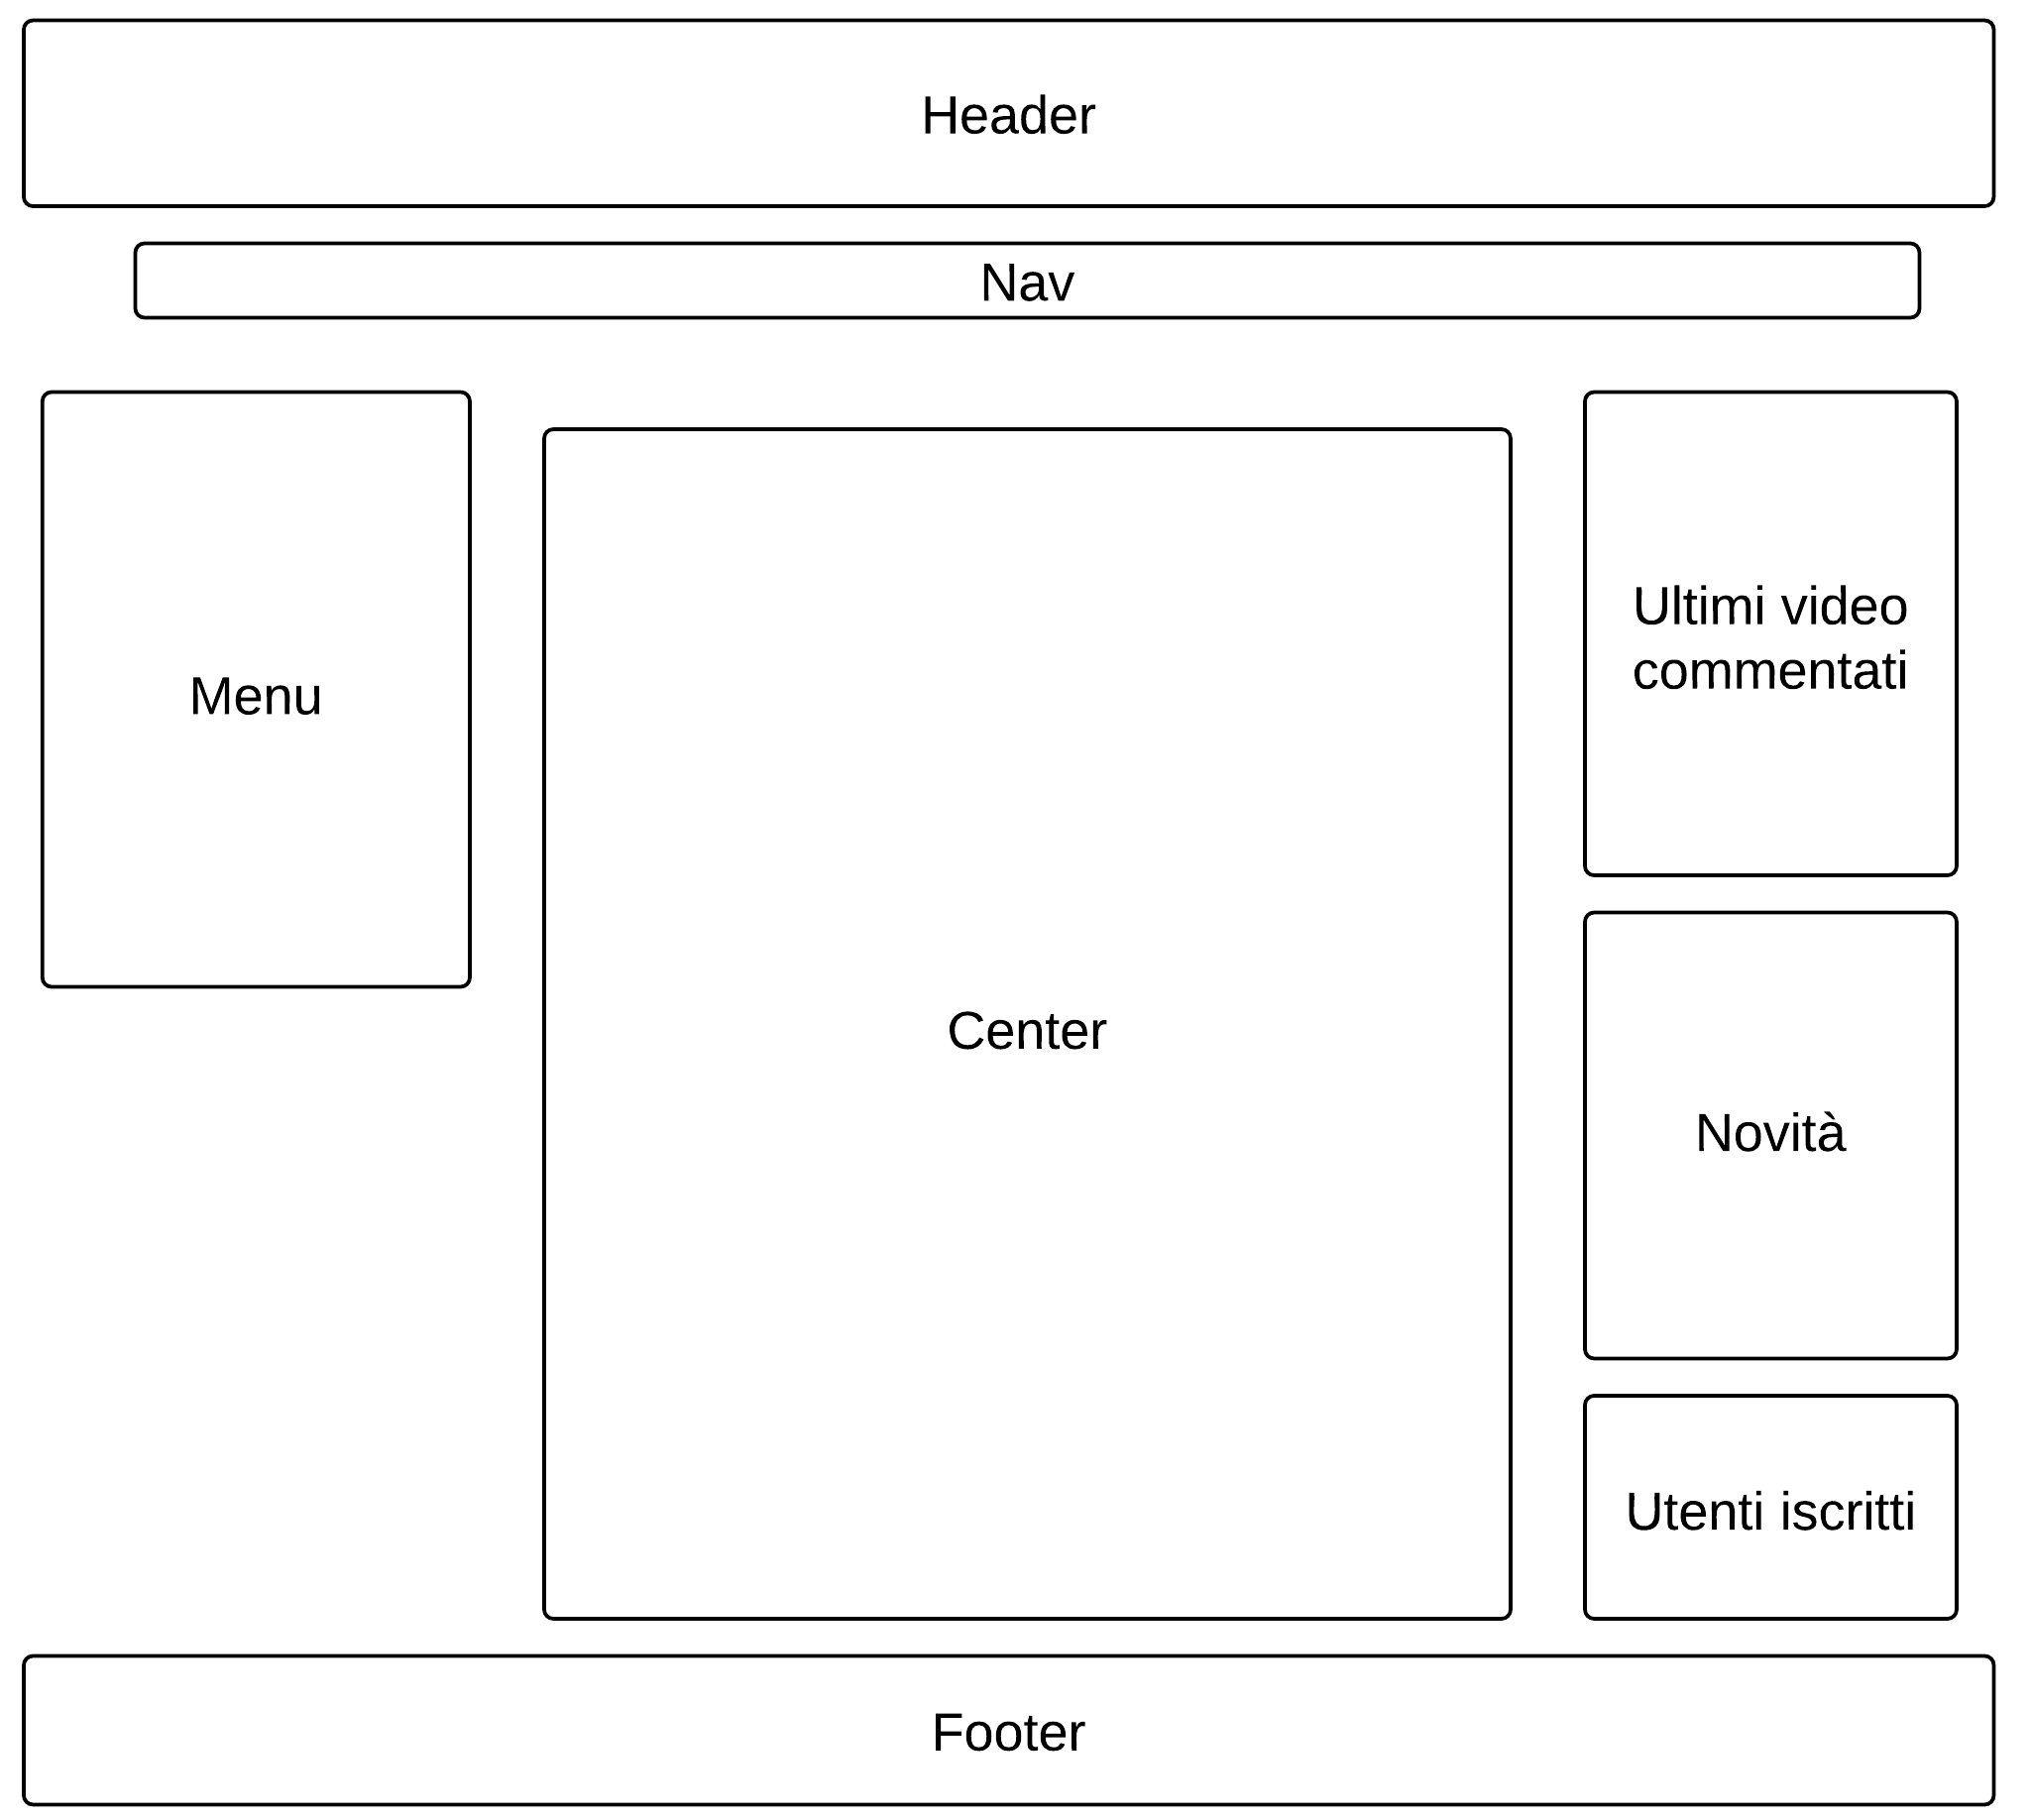
\includegraphics[scale=0.8]{images/baseLayout.png}
\caption{Schema layout base}
\end{figure}
\end{center}

L'Header è la parte superiore di presentazione del sito, troviamo poi il nav, parte molto importante perchè aiuta la navigazione indicando per ogni pagina la posizione corrente.\\
A destra è situto il Menu principale per la navigazione, mentre nel Center è presentato il contenuto fondamentale della pagina visualizzata. A sinistra vi sono delle parti informative sugli ultimi video commentati, sulle novità e gli utenti iscritti, mentre sotto a chiusura è posto il Footer.


\item \textbf{Layout per la stampa:}\\
 \textit{printStyle.css} 

\begin{center}
\begin{figure}[H]
\centering
%\includegraphics[scale=0.45]{clientClassDiagramm.png}
\caption{Schema layout per la stampa}
\end{figure}
\end{center}



\item \textbf{Layout per dispositivi smartphone:}\\
Per la visualizzazione del sito attraverso normali dispositivi come pc o portatili, viene applicato il foglio di del file \textit{smartStyle.css} 

\begin{center}
\begin{figure}[H]
\centering
%\includegraphics[scale=0.45]{clientClassDiagramm.png}
\caption{Schema layout smartphone}
\end{figure}
\end{center}

\end{itemize}



suddivisione pagina:\\
header\\
right(nav) center left(ultimi commentati, novità, utenti iscritti)\\
footer\\


\section{Reperibilità delle pagina dai motori di ricerca}

In un sito come quello presentato, è fondamentale il posizionamento assegnatogli dai diversi motori di ricerca. Tuttavia, diversamente da un sito tradizionale, un utente generico non sarà interessato a cercare "AllStreaming" (per esempio su Google), bensì è molto più probabile che cerchi il titolo del film o della serie a cui è interessato seguito dalla keyword "streaming".\\ 
Un esempio pratico potrebbe essere "Alla ricerca di Nemo streaming Ita"; per questo i metatag keyword presenti all'interno di ogni pagina film o serie, sono generati dinamicamente, prevedendo anche il titolo della stessa.

\section{Tecnologie/Struttura ??}
Lo cavemo?



\section{Validazioni}
xhtml
css
xml






\subsubsection{Client class }
\begin{center}
\begin{figure}[H]
\centering
%\includegraphics[scale=0.45]{clientClassDiagramm.png}
\caption{Client class diagram}
\label{ww-lists }
\end{figure}
\end{center}



\subsubsection{Server class }
\begin{center}
\begin{figure}[H]
\centering
%\includegraphics[scale=0.5]{serverClassDiagramm.png}
\caption{Server class diagram}
\label{ww-lists }
\end{figure}
\end{center}




\end{document}
